\chapter{Конструкторский раздел}

\section{IDEF0}

На рисунках \ref{img:IDEF00}-\ref{img:IDEF02} представлена IDEF0-диаграмма, описывающая работу межсетевого экрана.



\begin{figure}[h]
	\begin{center}
		{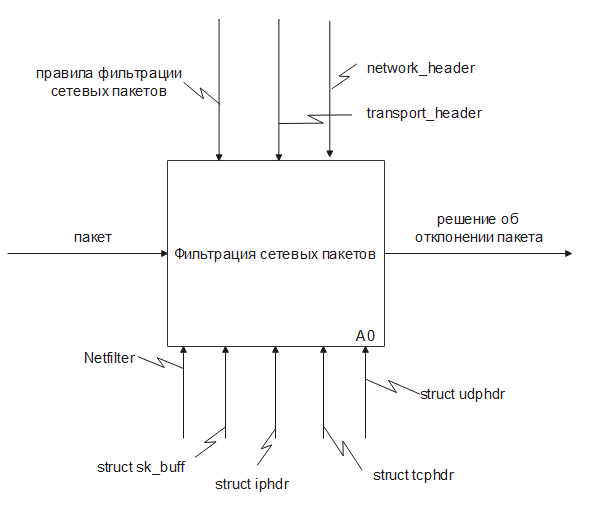
\includegraphics[scale = 1.5]{inc/img/IDEF00.png}}
		\caption{Фильтрация сетевых пакетов, верхний уровень}
		\label{img:IDEF00}
	\end{center}
\end{figure}


\clearpage
\begin{figure}[h!]
	\begin{center}
		{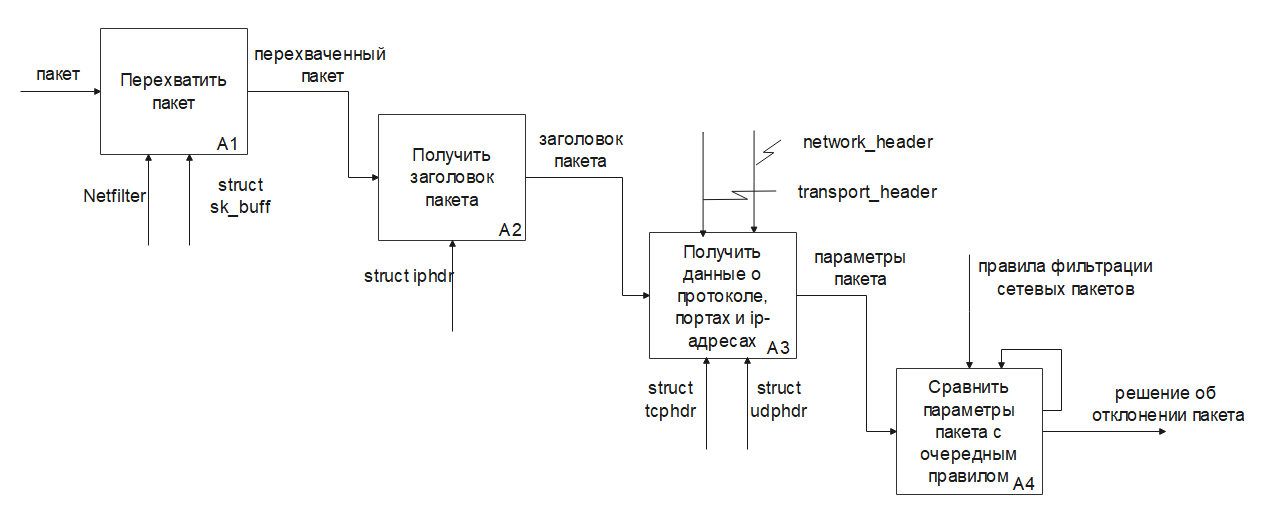
\includegraphics[scale = 0.9]{inc/img/IDEF02.png}}
		\caption{Фильтрация сетевых пакетов, нижний уровень}
		\label{img:IDEF02}
	\end{center}
\end{figure}

\section{Структура программного обеспечения}

Межсетевой экран должен быть реализован в виде загружаемого модуля ядра и работать в режиме ядра. Однако пользователь должен иметь возможность управлять работой межсетевого экрана и редактировать правила фильтрации, для чего необходимо разработать отдельное приложение, которое будет выполняется в режиме пользователя.

Структура программного обеспечения приведена на рисунке \ref{img:structure}.

\begin{figure}[h!]
	\begin{center}
		{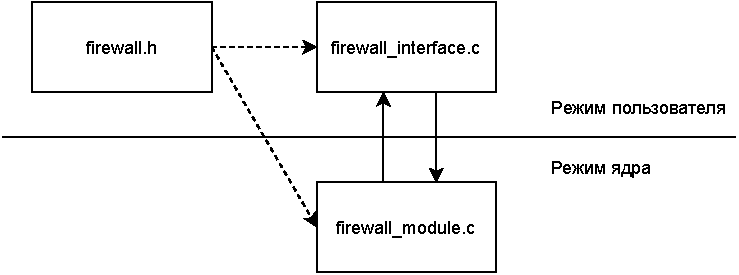
\includegraphics[scale = 1]{inc/img/structure.pdf}}
		\caption{Структура программного обеспечения}
		\label{img:structure}
	\end{center}
\end{figure}

\section{Алгоритм инициализации модуля}

На рисунке \ref{img:register} приведена схема алгоритма инициализации модуля.

%\clearpage
\begin{figure}[h!]
	\begin{center}
		{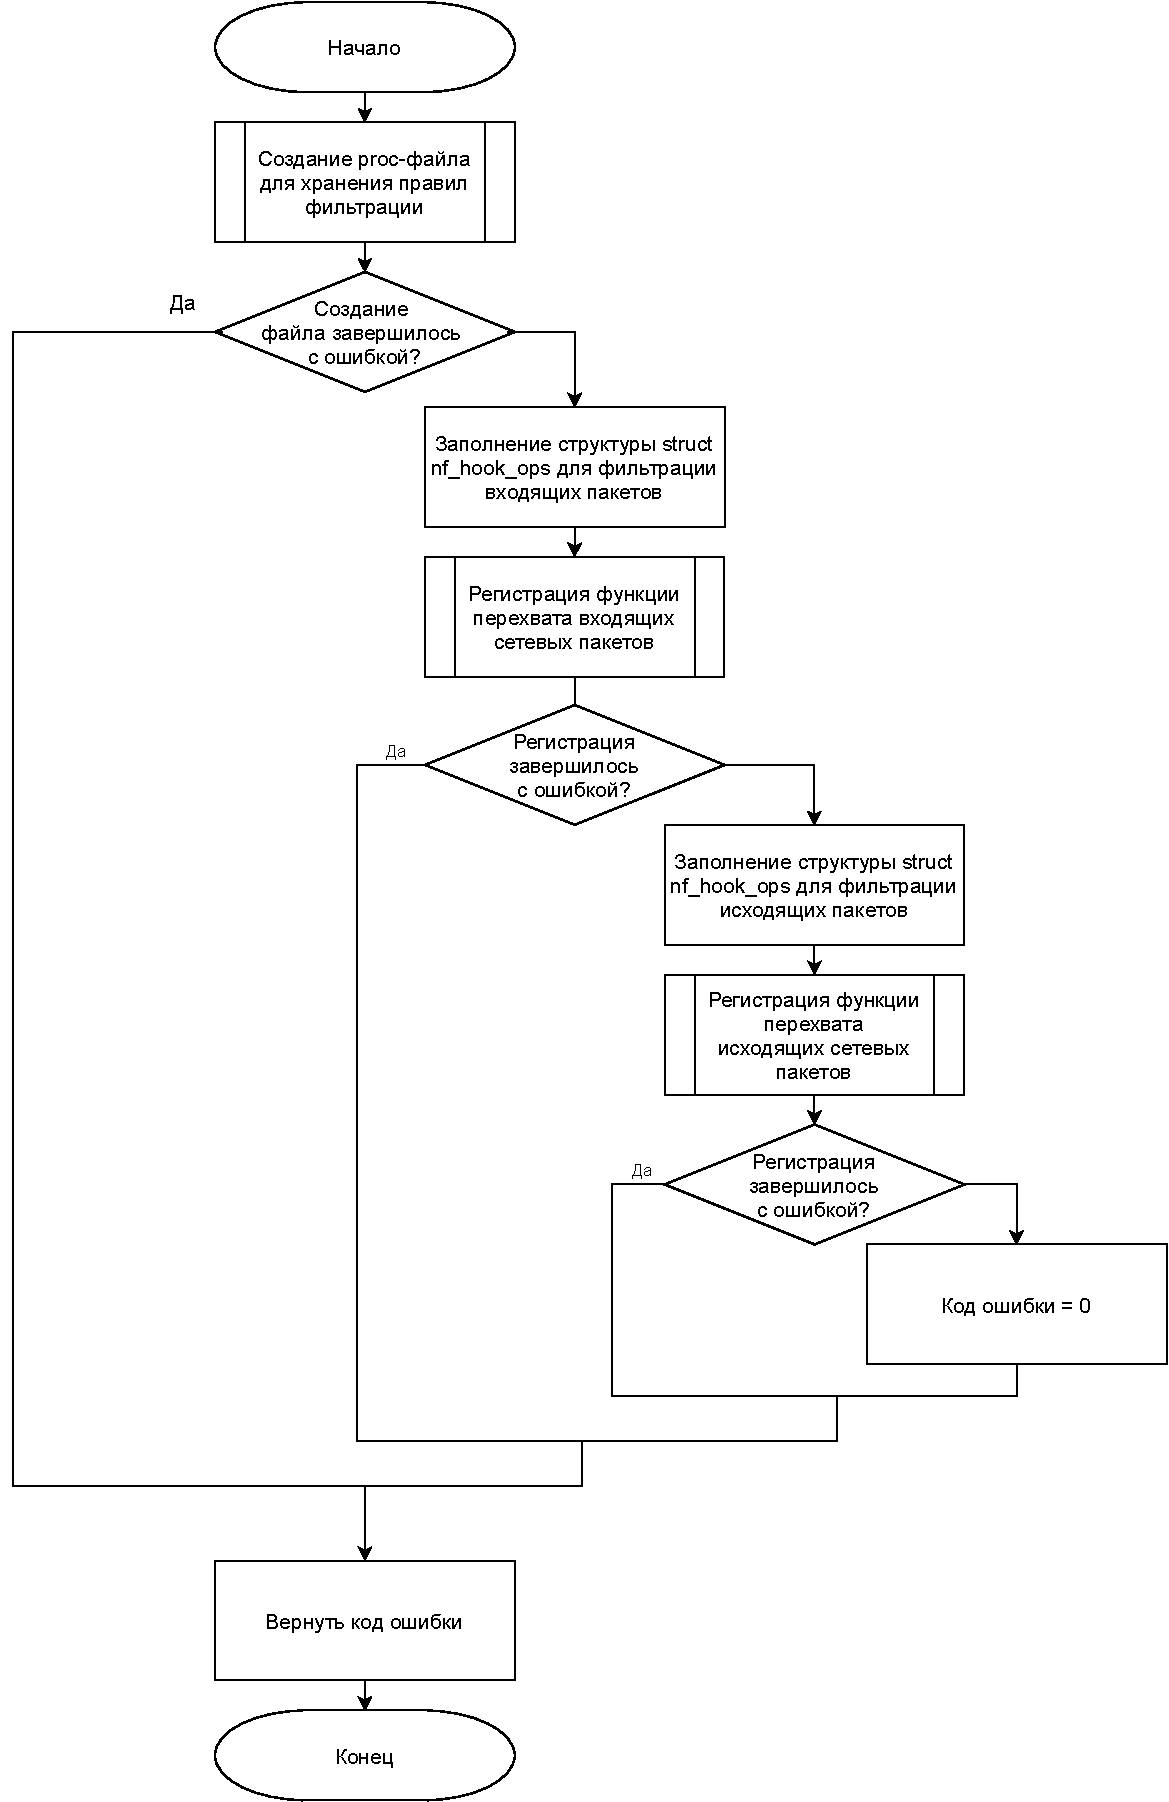
\includegraphics[scale = 0.65]{inc/img/register.pdf}}
		\caption{Алгоритм инициализации модуля}
		\label{img:register}
	\end{center}
\end{figure}


\section{Алгоритм фильтрации сетевых пакетов}

На рисунках \ref{img:filter-1}-\ref{img:filter-2} приведена схема алгоритма фильтрации на примере входящих сетевых пакетов.


%\clearpage
\begin{figure}[h!]
	\begin{center}
		{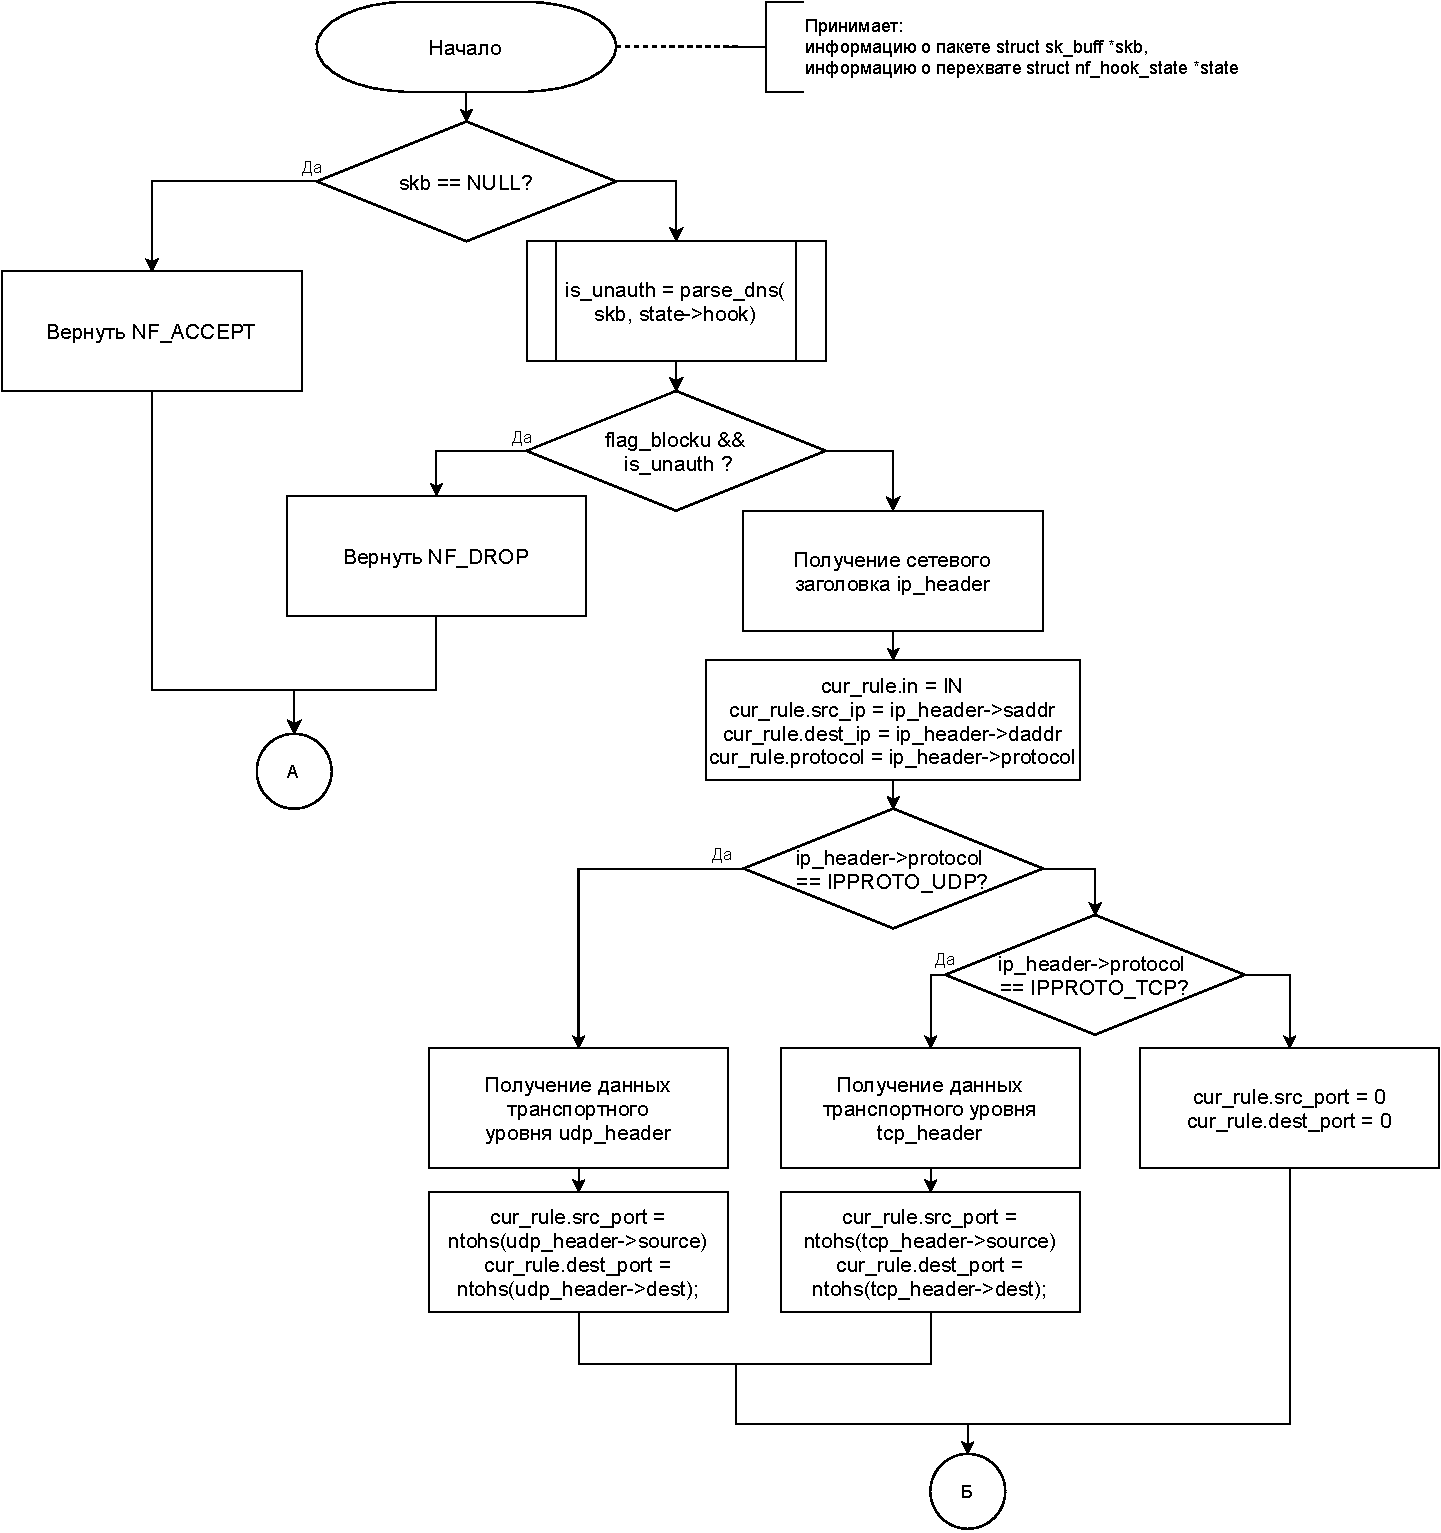
\includegraphics[scale = 0.7]{inc/img/filter-1.pdf}}
		\caption{Алгоритм фильтрации сетевых пакетов, начало.}
		\label{img:filter-1}
	\end{center}
\end{figure}

\clearpage
\begin{figure}[h!]
	\begin{center}
		{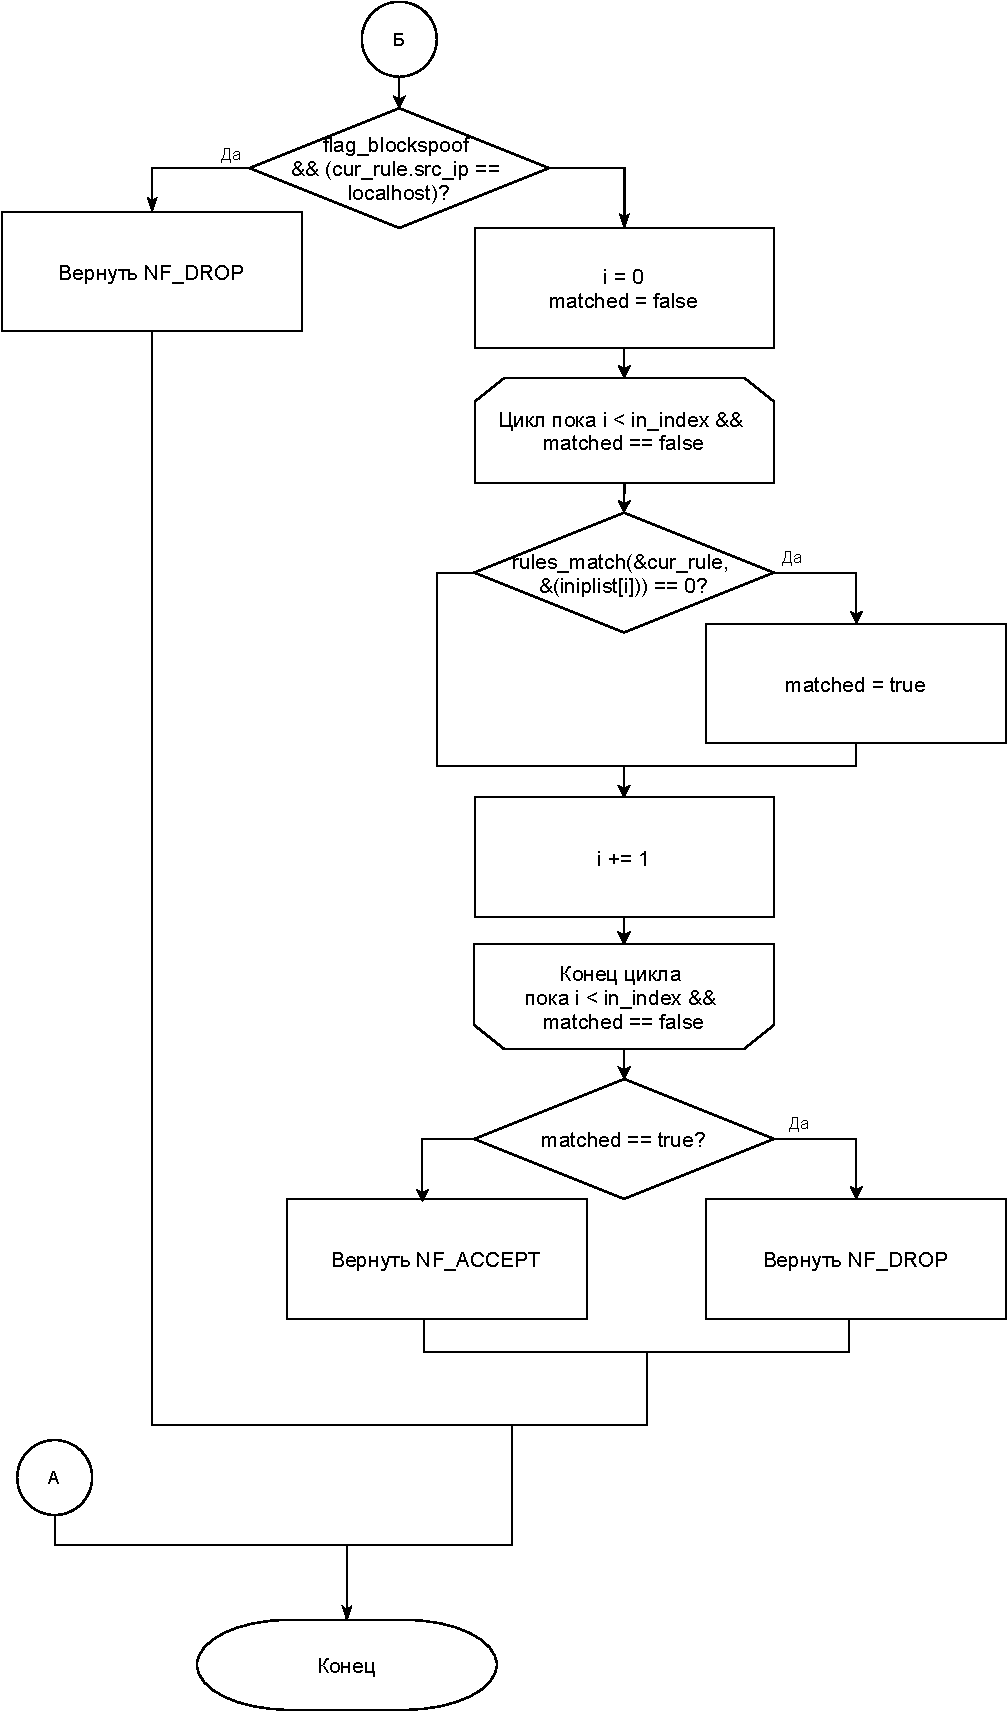
\includegraphics[scale = 0.85]{inc/img/filter-2.pdf}}
		\caption{Алгоритм фильтрации сетевых пакетов, конец.}
		\label{img:filter-2}
	\end{center}
\end{figure}

\clearpage
\section{Алгоритм проверки совпадения правил}

На рисунке \ref{img:compare} приведена схема алгоритма проверки совпадения правил, который применяется для определения того, удовлетворяет ли рассматриваемый пакет очередному правилу.

%\clearpage
\begin{figure}[h!]
	\begin{center}
		{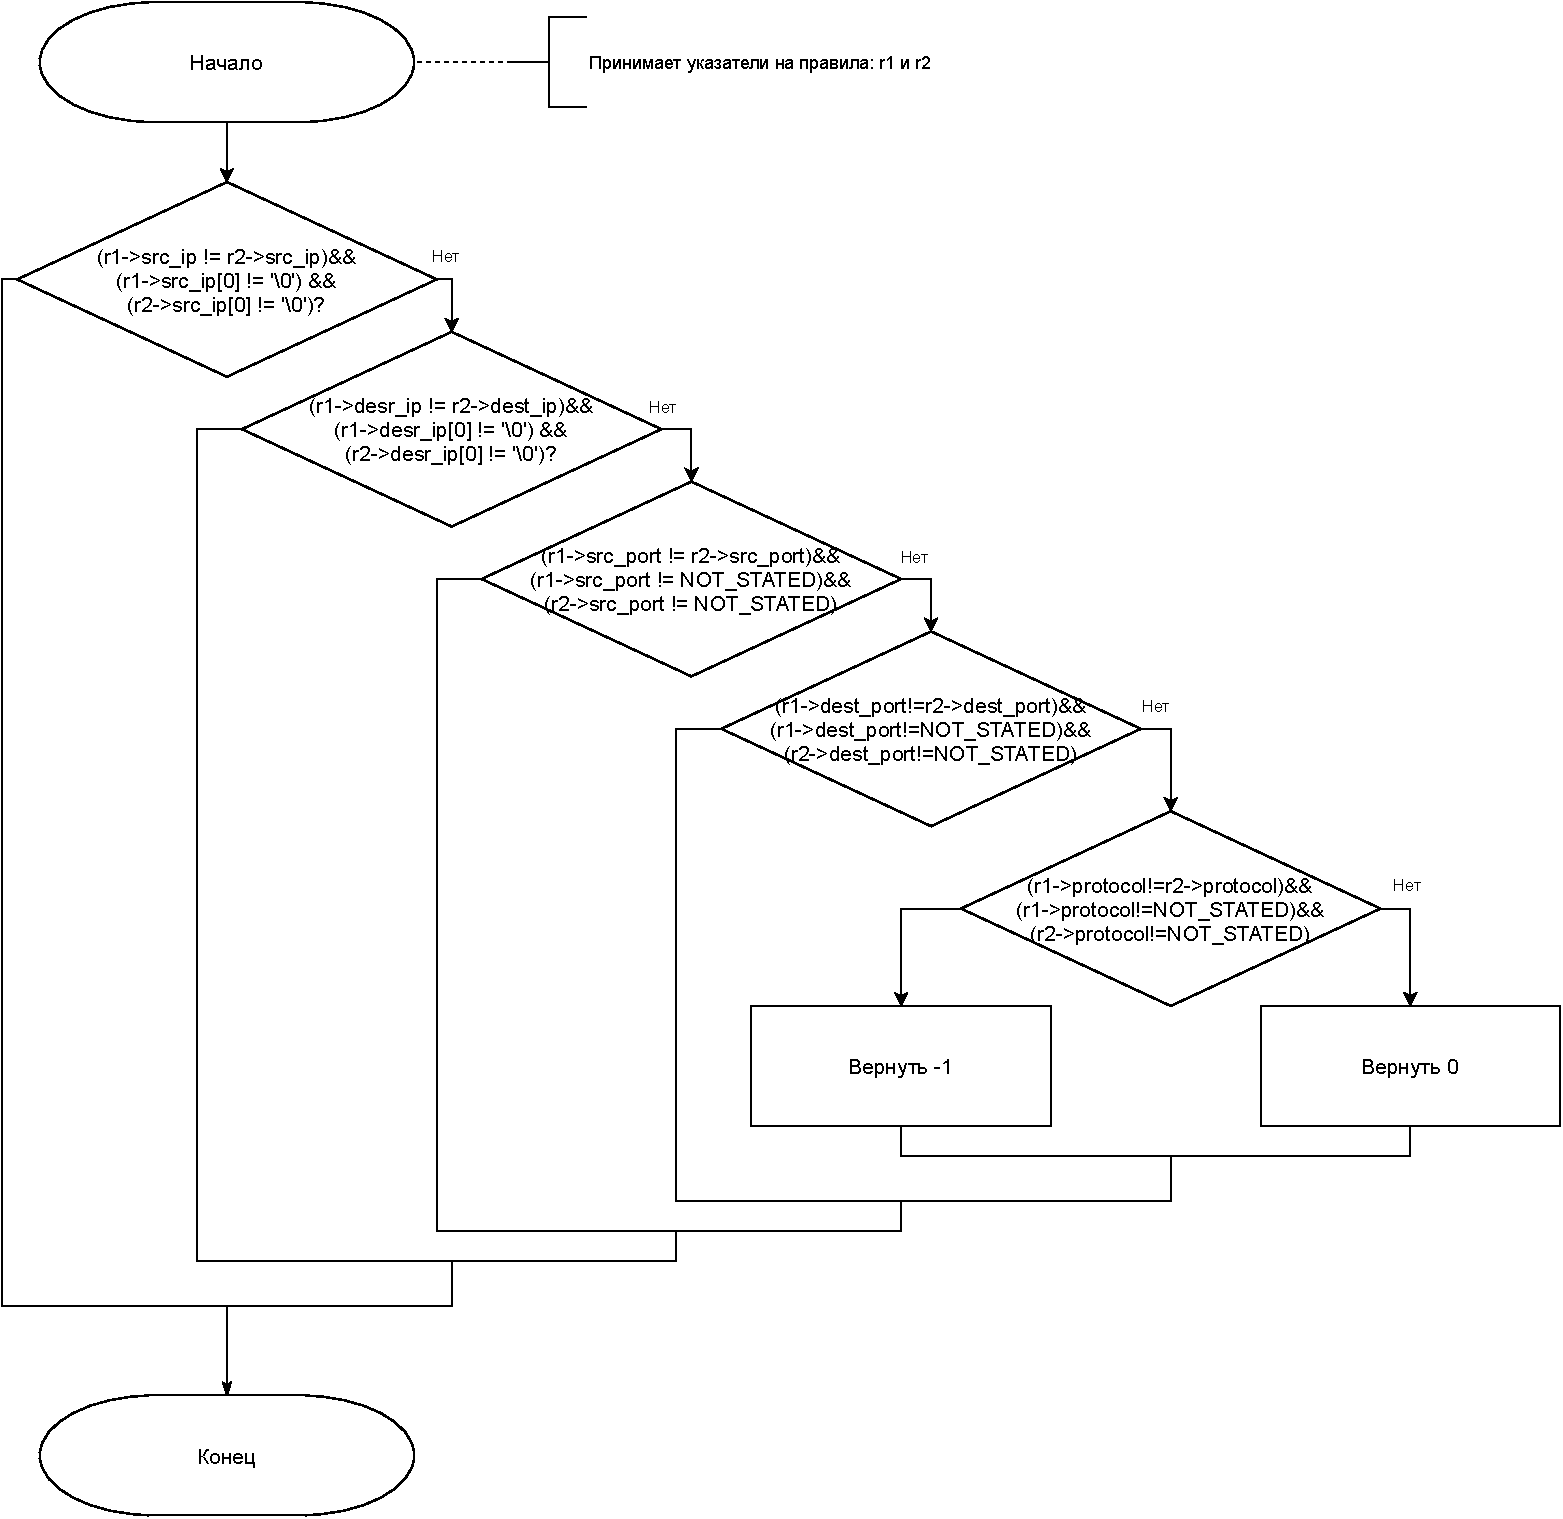
\includegraphics[scale = 0.65]{inc/img/compare.pdf}}
		\caption{Алгоритм проверки совпадения правил}
		\label{img:compare}
	\end{center}
\end{figure}

\clearpage
\section{Алгоритм вывода информации о DNS-пакете}

На рисунке \ref{img:parse_dns} приведена схема алгоритма вывода информации о DNS-пакете.

%\clearpage
\begin{figure}[h!]
	\begin{center}
		{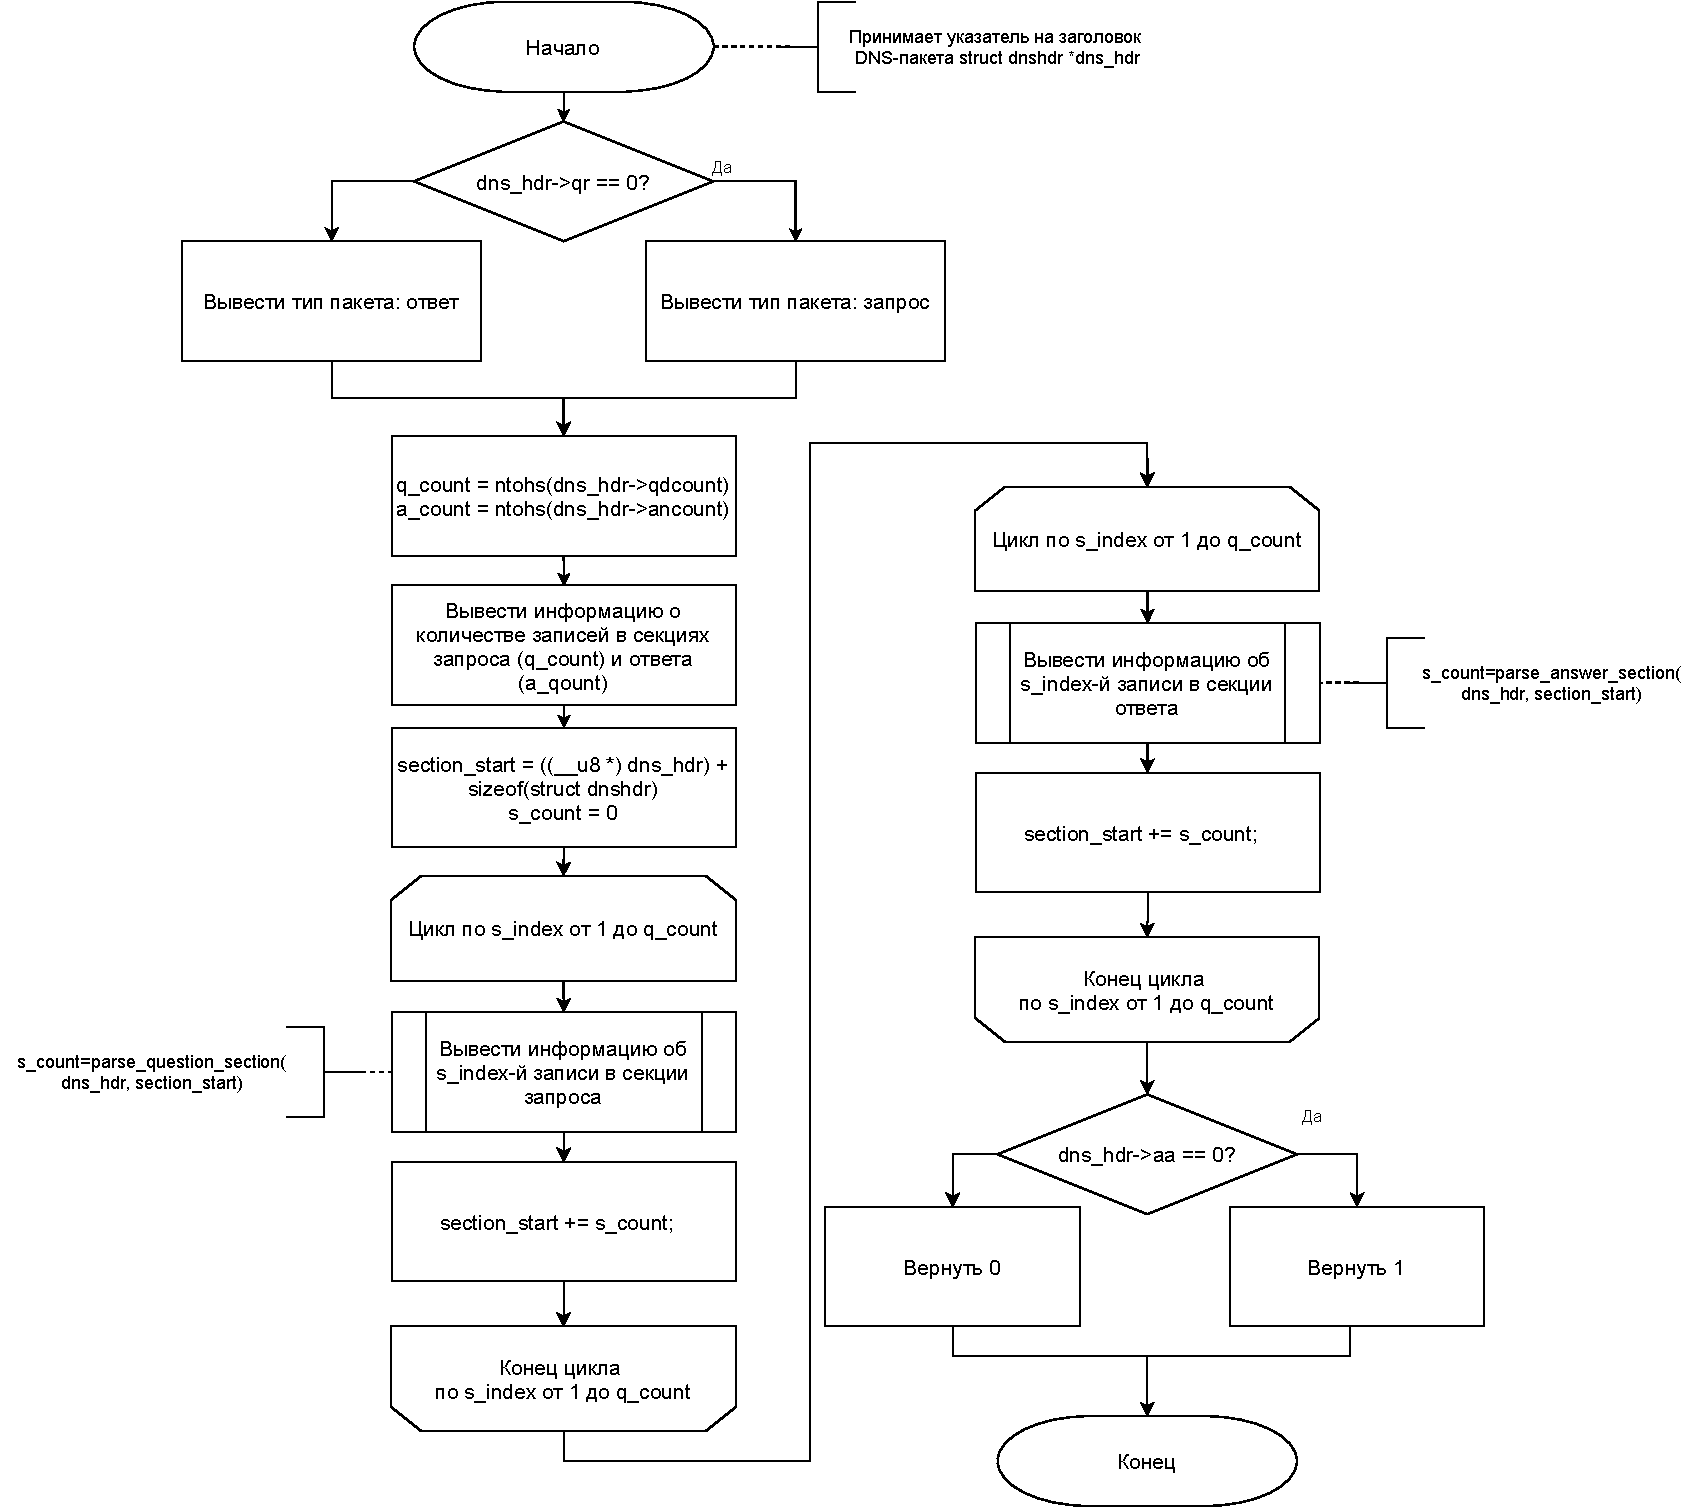
\includegraphics[scale = 0.62]{inc/img/dns.pdf}}
		\caption{Алгоритм вывода информации о DNS-пакете}
		\label{img:parse_dns}
	\end{center}
\end{figure}

